ee%\documentclass[11pt]{beamer}
\documentclass[ aspectratio=169]{beamer}
\usetheme{Warsaw}
%\usetheme{PaloAlto}
\usepackage[utf8]{inputenc}
\usepackage[french]{babel}
\usepackage[T1]{fontenc}
\usepackage{amsmath}
\usepackage{amsfonts}
\usepackage{amssymb}
\usepackage{graphicx}
\usepackage{pas-math}
\usepackage{lmodern}
\usepackage{fourier}
%\usepackage{algorithm}
\usepackage{dsfont}
\usepackage{algorithmic}
\usepackage[linesnumbered, french,onelanguage]{algorithm2e}
%\usepackage{libertine}
%\usepackage{chancery}
\usepackage{eulervm}

\usepackage[dvipsnames]{xcolor}
\DeclareMathAlphabet{\mathdsss}{U}{dsss}{m}{n}

\author{EGBAKOU Kodzovi David}
\title{Étude d'une stratégie de résolution du Jeu de Nim et conception d'un algorithme pour ledit jeu basé sur l'apprentissage automatique}
%\setbeamercovered{transparent} 
%\setbeamertemplate{navigation symbols}{} 
%\logo{} 
\institute{SCEI 18709} 
\date{} 
\subject{Algorithme du Jeu de Nim} 

\setbeamercolor{mine}{fg=White,bg= BlueViolet}

\begin{document}

\begin{frame}
\titlepage
\end{frame}

%\begin{frame}
%\tableofcontents
%\end{frame}

\begin{frame}
\tableofcontents[hideallsubsections]
\end{frame}

\section {Introduction}
\begin{frame}
\tableofcontents[hideothersubsections]
\end{frame}

\begin{frame}{Introduction}
		\begin{figure}[h]
			\centering
			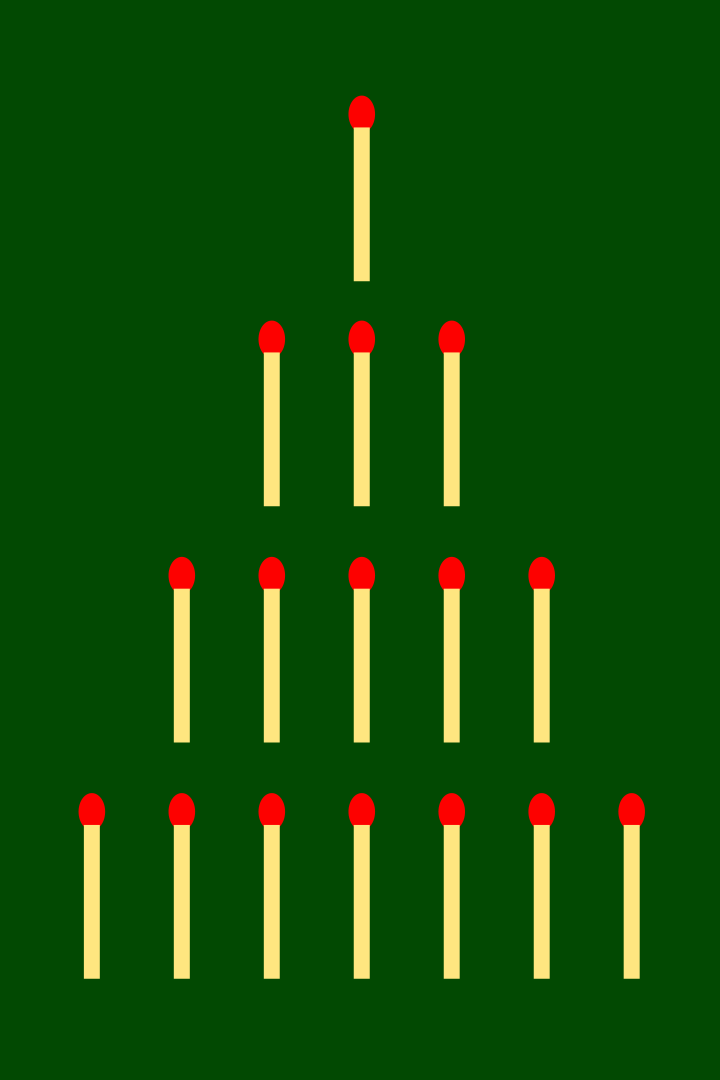
\includegraphics[scale=.15]{NimGame}
			\caption{Présentation du jeu de Nim}
		\end{figure}
\end{frame}
\subsection {Problématique}
\begin{frame}{Problématique}
Comment modéliser un algorithme assurant la victoire au jeu du Nim?
\end{frame}

\section {Analyse théorique}
\begin{frame}
\tableofcontents[hideothersubsections]
\end{frame}

	\subsection {Solution binaire}
	\begin{frame}
	La solution de résolution binaire se base sur la décomposition en binaire puis à partir d'un calcul à l'aide d'une \textit{somme digitale} on obtient une solution interprétable.\\
	Cette méthode se déroule en 4 étapes :
	\begin{itemize}
	\item Formation de la matrice binaire associée à la configuration 
	\item Calcul de la somme digitale de chaque colonne
	\item Vérification de la nature de la position du joueur 
	\end{itemize}
	\end{frame}
		
		\begin{frame}{Matrice associée}
		\subsubsection{Matrice associée}
		Soit une matrice $M$ de taille $(n,m)$. M est la matrice associée à la configuration du jeu à un instant donné\\
		On a : \\
		\begin{equation}
		 M =
		\begin{bmatrix}
		a_{11}&a_{12} & \dots & a_{1m}\\
		a_{21}&a_{22} & \dots & a_{2m}\\
		\vdots & \vdots & \ddots & \vdots \\
		a_{n1}& a_{n2} & \dots & a_{nm}
		\end{bmatrix}
		\end{equation}\\
		tel que $\forall i,j \in \left\lbrace 1,2,\dots ,n\right\rbrace , a_{ij} \in \{ 0 , 1\} $
		\end{frame}
		
		\begin{frame}{Somme digitale}
			\begin{block}{Définition: Somme digitale}
	La somme digitale est un opérateur défini sur l'ensemble des entiers. Elle consiste en une somme modulo 2.\\
	Elle sera notée dans la suite par $\oplus$
			\end{block}
		\end{frame}
		
		\begin{frame}
		Soit M la matrice associée à une position au jeu de Nim :\\
		Notons $Sd_{j}$ la somme digitale de la j\textsuperscript{ème} colonne. Alors on a 
		\begin{equation*}
		\forall j \text{<} m+1, Sd_{j} \equiv \left(\sum_{i=1}^n a_{ij}\right) \mod 2
		\end{equation*}
		Donc, la somme digitale appliquée à la matrice M est 
		$$
		a_{11}a_{12}\dots a_{1m} \oplus a_{21}a_{22}\dots a_{2m} \oplus \dots \oplus a_{n1}a_{n2}\dots a_{nm} = Sd_{1}Sd_{2}\dots Sd_{m}
		$$
		\end{frame}
		
		\begin{frame}{Somme digitale}
		Propriétés de la somme digitale:
		\begin{itemize}
		\item Associativité :
		$
		( a_{0}a_{1}\dots a_{n} \oplus b_{0}b_{1}\dots b_{n})\oplus c_{0}c_{1}\dots c_{n} = a_{0}a_{1}\dots a_{n} \oplus (b_{0}b_{1}\dots b_{n}\oplus c_{0}c_{1}\dots c_{n})
		$
		\item Commutativité : 
		$
		a_{0}a_{1}\dots a_{n} \oplus b_{0}b_{1}\dots b_{n}=b_{0}b_{1}\dots b_{n} \oplus a_{0}a_{1}\dots a_{n}
		$
		\item Existence d'un élément neutre : $a_{0}a_{1}\dots a_{n} \oplus 0 = a_{0}a_{1}\dots a_{n}$
		\item Existence d'un opposé :
		$
		\forall a_{0}a_{1}\dots a_{n}, \exists b_{0}b_{1}\dots b_{n} \in \mathbb{N}, a_{0}a_{1}\dots a_{n} \oplus b_{0}b_{1}\dots b_{n}=0
		$
		\end{itemize}
		\end{frame}
		
		\begin{frame}
		\begin{block}{Théorème de Bouton}
		Si la position dans laquelle se trouve un joueur possède une somme digitale non nulle, alors il se trouve en position gagnante ; sinon, ce sera son adversaire qui sera en position gagnante.
		\end{block}
		 
		 
		\end{frame}
		
		\begin{frame}
		Le théorème de Bouton repose sur deux lemmes très important qui permettent de donner un sens à la nature de la position\\
		Soit $x_{i}$ le nombre d'allumettes de la $i^{ème}$ ligne avec $i$ un entier compris entre $1$ et $n$ ; et $y_{1}, y_{2},\dots, y_{n}$ les lignes après qu'un joueur est joué.\\
		 Notons $Sd_{b} = x_{1} \oplus x_{2}\oplus \dots \oplus x_{n}$ et $Sd_{f} = y_{1} \oplus y_{2}\oplus \dots \oplus y_{n}$
		 \end{frame}
		 
		\begin{frame}
		\begin{exampleblock}{Lemme 1}
		Si un joueur se trouve en position perdante, alors tous ses coups mèneront son adversaire en position gagnante
		\end{exampleblock}
		Autrement si $Sd_{b}= 0$ alors $Sd_{f} \neq 0$
		\begin{exampleblock}{Lemme 2}
		Si le joueur se trouve en position gagnante, il existe au moins un coup qui nous permet de mettre notre adversaire dans une position perdante.
		\end{exampleblock}
		C'est-à-dire, si $Sd_{b} \neq 0$ alors il existe  un mouvement tel que $Sd_{f}= 0$
		\end{frame}
		\subsection{Approche par les graphes}
		\begin{frame}{Approche par les graphes}
		\begin{figure}[h]
			\centering
			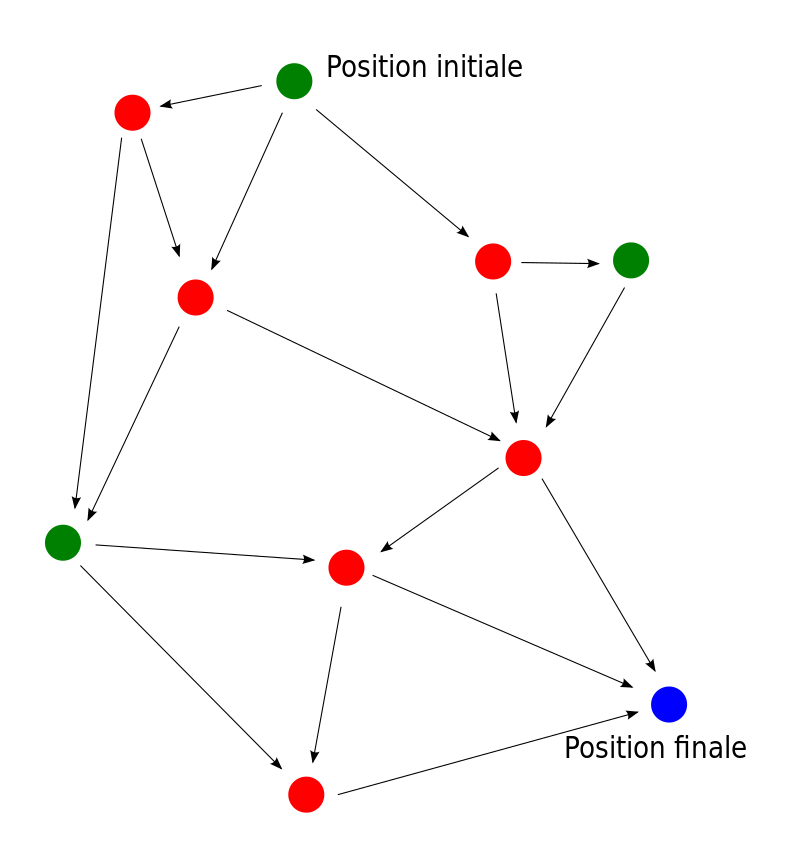
\includegraphics[scale=0.16]{JeuNim}
			\caption{Représentation graphique du jeu de Nim}
		\end{figure}		
		\end{frame}
		\begin{frame}{Approche par les graphes}
		Le jeu de Nim admet une représentation au travers d'un graphe orienté sans circuit. Chaque sommet désigne une position possible au cours de la partie\\
		Désignons par $x$ la position actuelle, soit $y$ une image de $x$ et $\Phi \left( x\right) $ l'ensemble des images de $x$
		\end{frame}
		
		\begin{frame}
		\begin{block}{Noyau d'un graphe}
		Le noyau $K $ d'un graphe est l'ensemble des sommets qui vérifient:
		\begin{itemize}
		\item $ x \in K \Longrightarrow \Phi \left( x \right) \bigcap K = \emptyset$
		\item $ x \notin K \Longrightarrow \Phi \left( x \right) \bigcap K \neq \emptyset$
		\end{itemize}
		\end{block}
		D'après le Lemme 2, $ K$ désigne l'ensemble des positions perdantes dans une partie
		\end{frame}
		
		\section{Travail Pratique}
		\begin{frame}
\tableofcontents[hideothersubsections]
\end{frame}
\subsection{Définition de l'environnement de Jeu}
Définition de la class NimEnv en utilisant un certain nombre de fonction
\begin{itemize}
    \item \texttt{\_\_init\_\_(self, seed=None) $\rightarrow$ None}
    \item \texttt{check\_valid(self, action) $\rightarrow$ bool}
    \item \texttt{step(self, action) $\rightarrow$ (self.heaps, self.end, self.winner)}
    \item \texttt{observe(self) $\rightarrow$ (self.heaps, self.end, self.winner)}
    \item \texttt{reward(self, player=0) $\rightarrow$ float}
    \item \texttt{reset(self, seed=None) $\rightarrow$ self.heaps.copy()}
    \item \texttt{render(self, simple=False) $\rightarrow$ None}
\end{itemize}

\subsection{Définition de l'agent optimal}
		
		\begin{algorithm}
\caption{Algorithme somme digitale}
\KwData{Piles}
\KwResult{un entier représentant le résultat de la somme digitale}
Initialiser $nim=0$ \;
\For{chaque éléments i de la Piles}{
	$nim\longleftarrow ni$m XOR $i$ \;}
	Retourne la valeur finale de nim
\end{algorithm}

\begin{frame}

\end{frame}

		\subsection {Apprentissage par Q-learning}
		\begin{frame}
		Le Q-learning est un algorithme d'apprentissage renforcée se basant sur trois étapes centrales à savoir: 
		\begin{itemize}
		\item \textbf{Connaître} : définir une fonction action-valeur Q
		\item \textbf{Renforcement des connaissances} : Mettre à jour la fonction Q
		\item \textbf{Agir} : Adopter une stratégie d'action 
		\end{itemize}
		\end{frame}
		
				
		\begin{algorithm}
\caption{Algorithme Q-learning}
\KwData{$A$, $S$, $\alpha$: taux d'apprentissage, $\gamma$: facteur d'actualisation, $\epsilon \in \mathbb{R}^{*}_{+}$}
\KwResult{Une $Q$-table contenant les $Q$-valeurs d'états et d'actions de l'agent}
Initialiser $Q(s,a)$ de façon aléatoire pour tout $(s,a) \in A \times S$, $i = 1$ \;
\For{chaque épisode}{
	Initialiser $s$\;
	\For{chaque étape $t$ de l'épisode}{
		Choisir l'action $a$ en utilisant \textbf{l'algorithme $\epsilon$-greedy}\;
		Effectuer l'action $a$, et recevoir la récompense $r$, et observer le nouvel état $s'$\;
		$Q_{t+1}(s,a) \leftarrow Q_{t}(s,a) + \alpha \left[ r + \gamma \max_{a' \in A} Q_{t}(s',a') - Q_{t}(s,a) \right]$, $s \leftarrow s'$
	}
}
\end{algorithm}

		\begin{algorithm}
		%\begin{Large}
\caption{Algorithme $\epsilon$-greedy}
\KwData{$Q$-table, $s \in S, \epsilon \in \mathbb{R}^{*}_{+}$}
\KwResult{Action choisie $a$}
$\eta \leftarrow$ un nombre aléatoire dans $\left[ 0, 1 \right]$\;
\eIf{$\eta$ < $\epsilon$}{
    $a \leftarrow$ action aléatoire dans $A$\;
}{
    $a \leftarrow \max_{a' \in A} Q(s, a')$\;
}
Retourne l'action $a$ sélectionnée\;
%\end{Large}
\end{algorithm}

   \begin{frame}
		   \begin{figure}
      \centering
 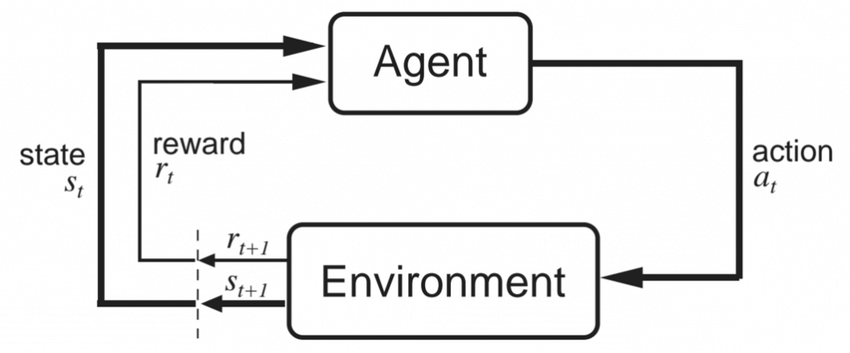
\includegraphics[scale=0.37]{Apprentissage-par-renforcement}
   \end{figure}
   \end{frame}
   \begin{frame}
   
   \end{frame}
	
\section{Résultats}	
\begin{frame}
\tableofcontents[hideothersubsections]
\end{frame}

\subsection{Indicateur de performance}
\begin{frame}
La performance est définie par:
\begin{itemize}
\item Mean reward
\item $M_{opt}$ tel que: $$M_{opt}= \frac{N_{win}-N_{lose}}{N}$$ avec N=500
\item $M_{rand}$
\end{itemize}
\end{frame}

\subsection{Résultats}

		\begin{frame}{Résultats}
		\begin{figure}[h]
			\centering
			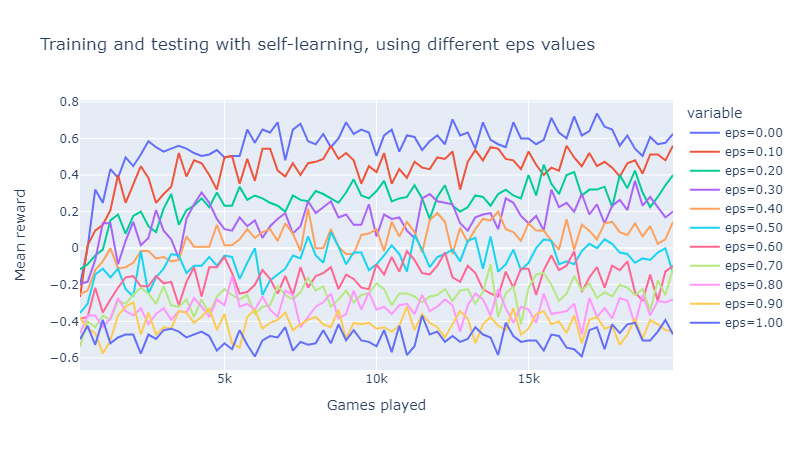
\includegraphics[scale=0.44]{newplot00}
			%\caption{Présentation du jeu de Nim}
		\end{figure}
		\end{frame}
		\begin{frame}{Résultats}
		\begin{figure}[h]
			\centering
			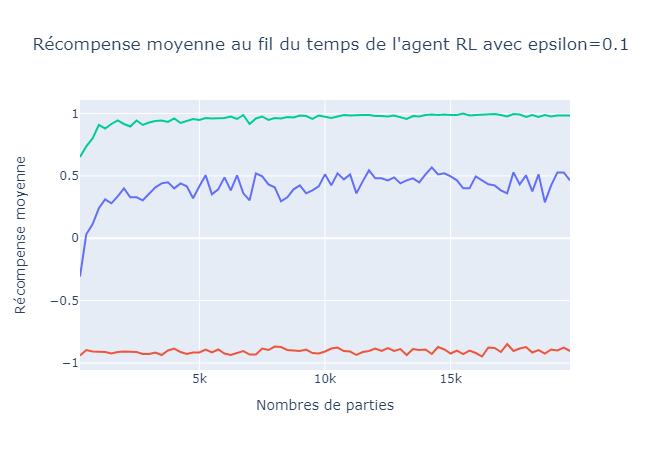
\includegraphics[scale=0.44]{newplot0}
			%\caption{Présentation du jeu de Nim}
		\end{figure}
		\end{frame}
		\begin{frame}
Pour rendre l'agent plus performant on fait décroître progressivement $\epsilon$, le taux d'exploration 
Ainsi, $$\epsilon(n) = \max \left\{\epsilon_{\min}, \epsilon_{\max} \left(1 - \frac{n}{n^*} \right) \right\}.$$

\end{frame}
		\begin{frame}{Résultats}
		\begin{figure}[h]
			\centering
			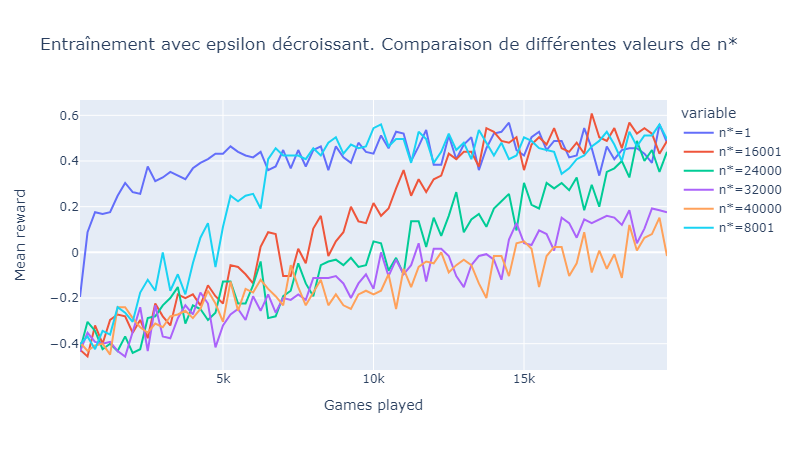
\includegraphics[scale=0.44]{newplot}
			%\caption{Présentation du jeu de Nim}
		\end{figure}
		\end{frame}	
				\begin{frame}{Résultats}
		\begin{figure}[h]
			\centering
			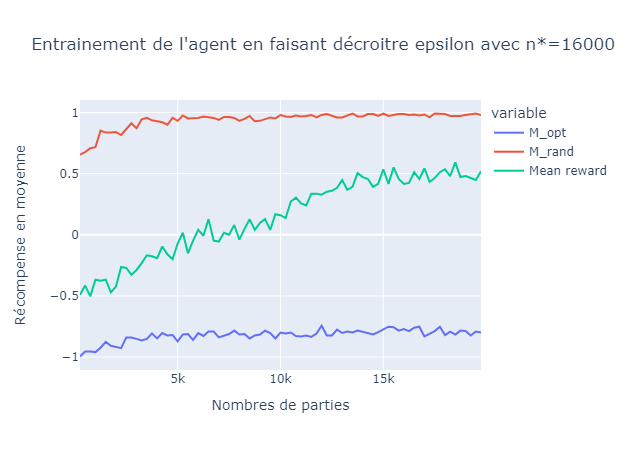
\includegraphics[scale=0.44]{newplot1}
			%\caption{Présentation du jeu de Nim}
		\end{figure}
		\end{frame}	
\begin{frame}{Conclusion}
		   \begin{figure}
      \centering
 
\includegraphics[scale=0.38]{Merci pour votre attention}
   \end{figure}
   \end{frame}	
\begin{frame}

Considérons $sd_{b}$ et $sd_{f}$ défini plutôt et admettons que le joueur prenne une/des allumette(s) dans la ligne $k$: $\forall i \neq k, x_{i} = y_{i}$ tandis que $x_{k} > y_{k}$. En appliquant les propriétés de $\oplus$ (associativité, commutativité et que $x \oplus x = 0$), nous obtenons :

\begin{align*}
sd_{f} &= 0 \oplus sd_{f} \\
&= sd_{b} \oplus sd_{b} \oplus sd_{f} \\
&= sd_{b} \oplus (x_{1} \oplus x_{2} \oplus ... \oplus x_{n} \oplus y_{1} \oplus y_{2} \oplus ... \oplus y_{n}) \\
&= sd_{b} \oplus (x_{1} \oplus y_{1}) \oplus (x_{2} \oplus y_{2}) \oplus ... \oplus (x_{k} \oplus y_{k}) \oplus ... \oplus (x_{n} \oplus y_{n}) \\
&= sd_{b} \oplus 0\oplus ...\oplus (x_{k} \oplus y_{k})\oplus ...\oplus 0 \\
&= sd_{b} \oplus x_{k} \oplus y_{k} \quad (1)
\end{align*}

Par récurrence à partir des 2 lemmes on obtient le théorème de Bouton

\end{frame}

\begin{frame}{Annexe 1 : Démonstration}

\textbf{Démonstration Lemme 1:} \\
Comme $sd_{b}=0$, alors $sd_{f}=x_{k} \oplus y_{k}$. Si le joueur modifie le nombre d'allumettes dans la ligne $k$ et étant donné que $x_{k} \neq y_{k}$, alors $sd_{f} \neq 0.$\\
\end{frame}

\begin{frame}{Annexe 1 : Démonstration}
\textbf{Démonstration du Lemme 2:} \\
Soit $d$ la position du premier chiffre non nul de $sd_{b}$ en commençant par la gauche. Prenons $k$ tel que le $d^{ieme}$ bit de $x_{k}$ est également non nul (k existe sinon le $d^{ieme}$ bit de $sd_{b}$ vaudrait 0).\\
Posons $y_{k}=sd_{b} \oplus x_{k}$, alors $y_{k}<x_{k}$.\\
Tous les bits se trouvant à gauche de $d$ sont semblables dans $x_{k}$ et $y_{k}$. Le $d^{ieme}$ bit qui est un 1 devient un 0 en faisant diminuer la valeur de $2^{d}$.\\
Peu importe quels sont les changements apportés sur les bits à droite de $d$, ils ne créeront en aucun cas un changement supérieur à $2^{d-1}$. Celui qui joue est en mesure de prendre $x_{k}-y_{k}$ allumettes de la ligne $k$ et donc:
\begin{align*}
sd_{f} &= sd_{b} \oplus x_{k} \oplus y_{k} \\
&= sd_{b} \oplus x_{k} \oplus (sd_{b} \oplus x_{k}) \\
&= 0
\end{align*}

\end{frame}


\begin{frame}{Annexe 2: Code python}
		   \begin{figure}
      \centering
 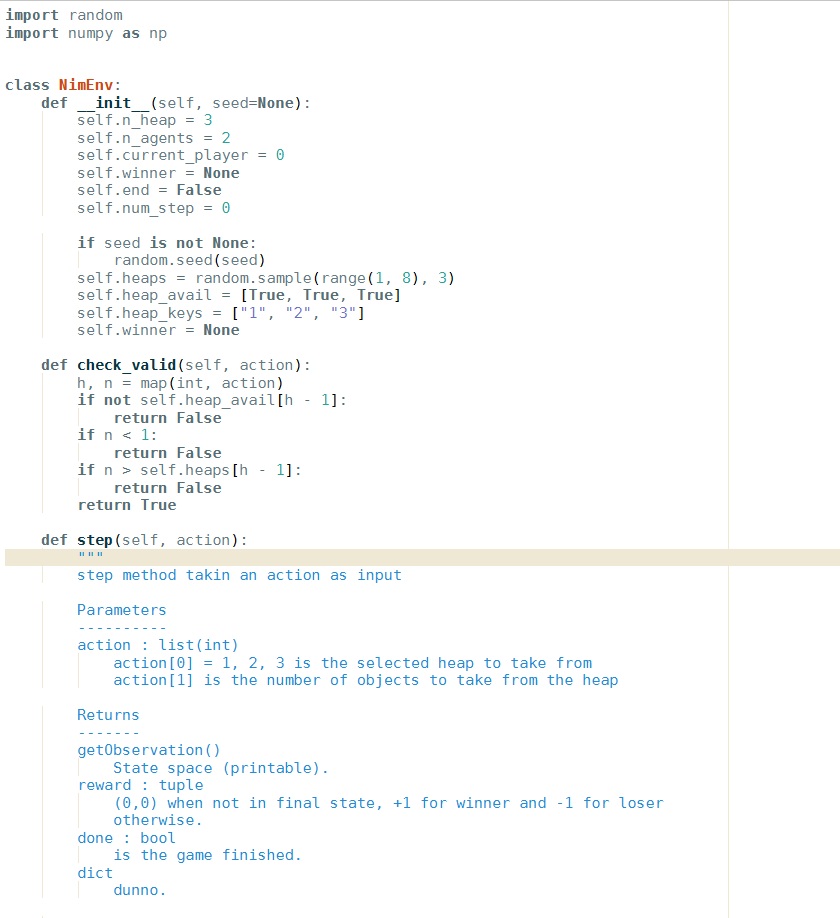
\includegraphics[scale=0.25]{Capture d'écran 2024-06-09 175311}
   \end{figure}
   \end{frame}
   
   
\begin{frame}{Annexe 2: Code python}
   \begin{figure}   
      \centering 
       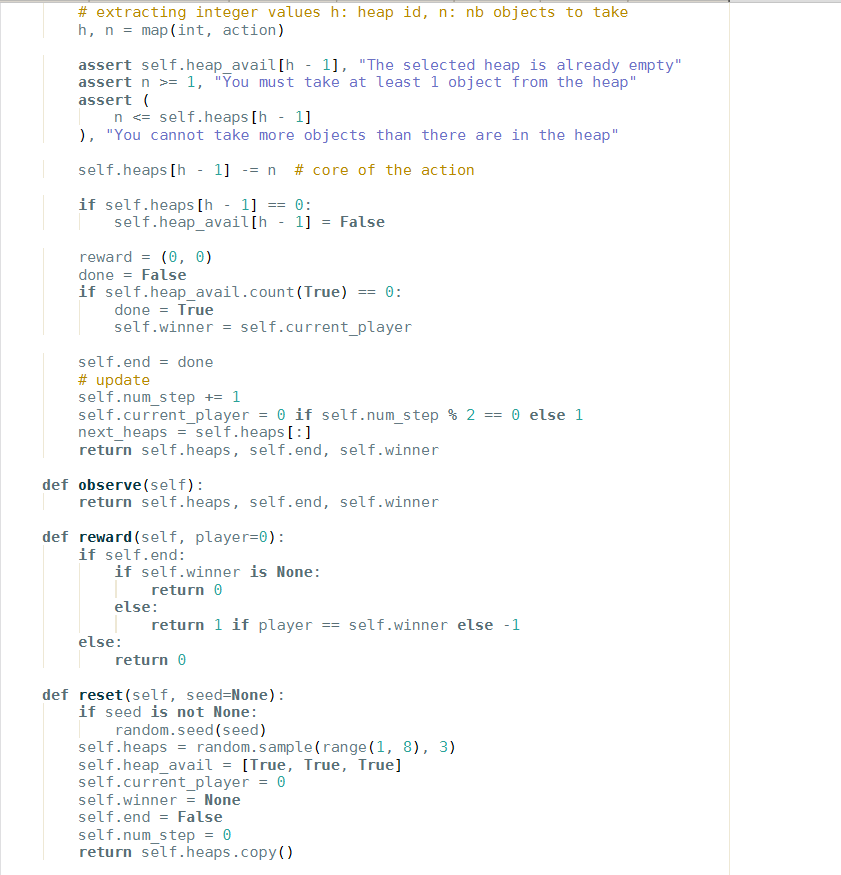
\includegraphics[scale=0.25]{Capture d'écran 2024-06-09 175405}
       \end{figure}
		\end{frame}
		
\begin{frame}{Annexe 2: Code python}
		\begin{figure}[h]
			\centering
			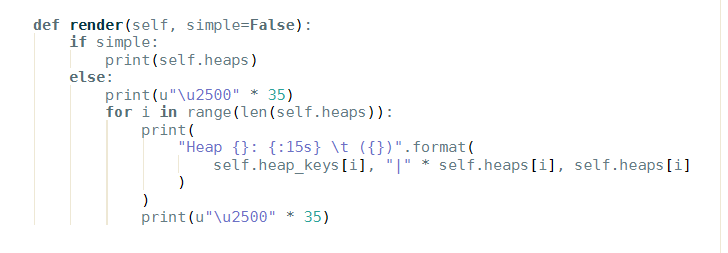
\includegraphics[scale=0.6]{Capture d'écran 2024-06-09 175420}
			%\caption{Présentation du jeu de Nim}
		\end{figure}
		\end{frame}
	
\begin{frame}{Annexe 2 : code python}
		   \begin{figure}
      \centering
 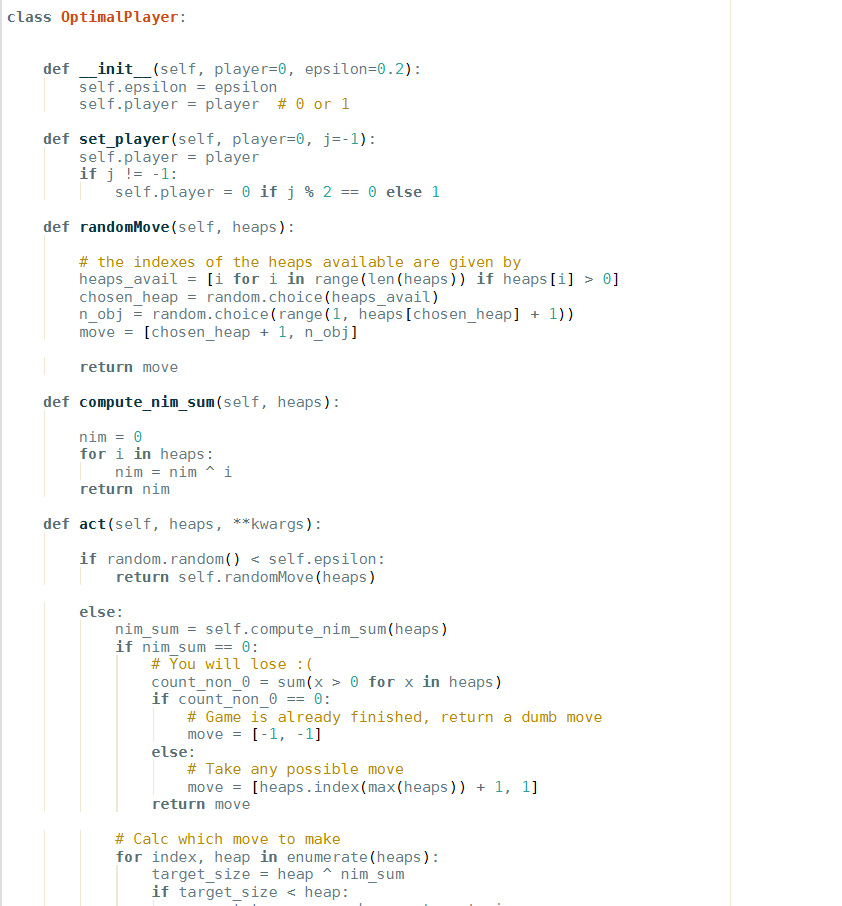
\includegraphics[scale=0.25]{Capture d'écran 2024-06-09 175524}
   \end{figure}
   \end{frame}
 
 \begin{frame}{Annexe 2 : code python}
   \begin{figure}   
      \centering 
       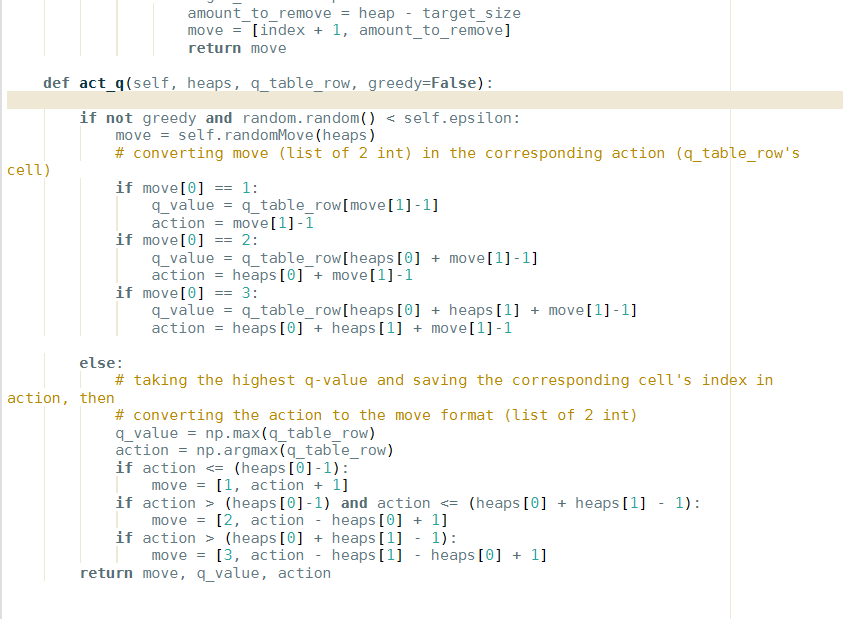
\includegraphics[scale=0.25]{Capture d'écran 2024-06-09 175548}
       \end{figure}
		\end{frame}
		
\begin{frame}{Annexe 2 : code python}
		   \begin{figure}
      \centering
 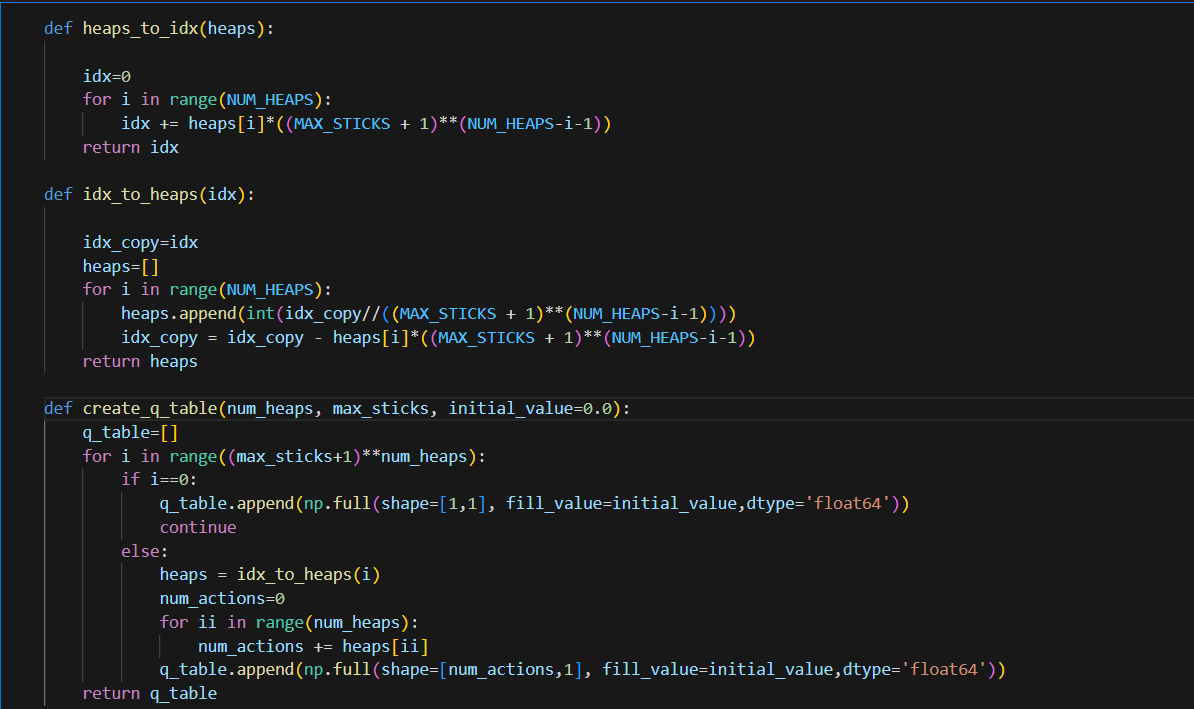
\includegraphics[scale=0.37]{Capture d'écran 2024-06-09 180514}
   \end{figure}
   \end{frame}			

\begin{frame}{Annexe 2 : code python}
		   \begin{figure}
      \centering
 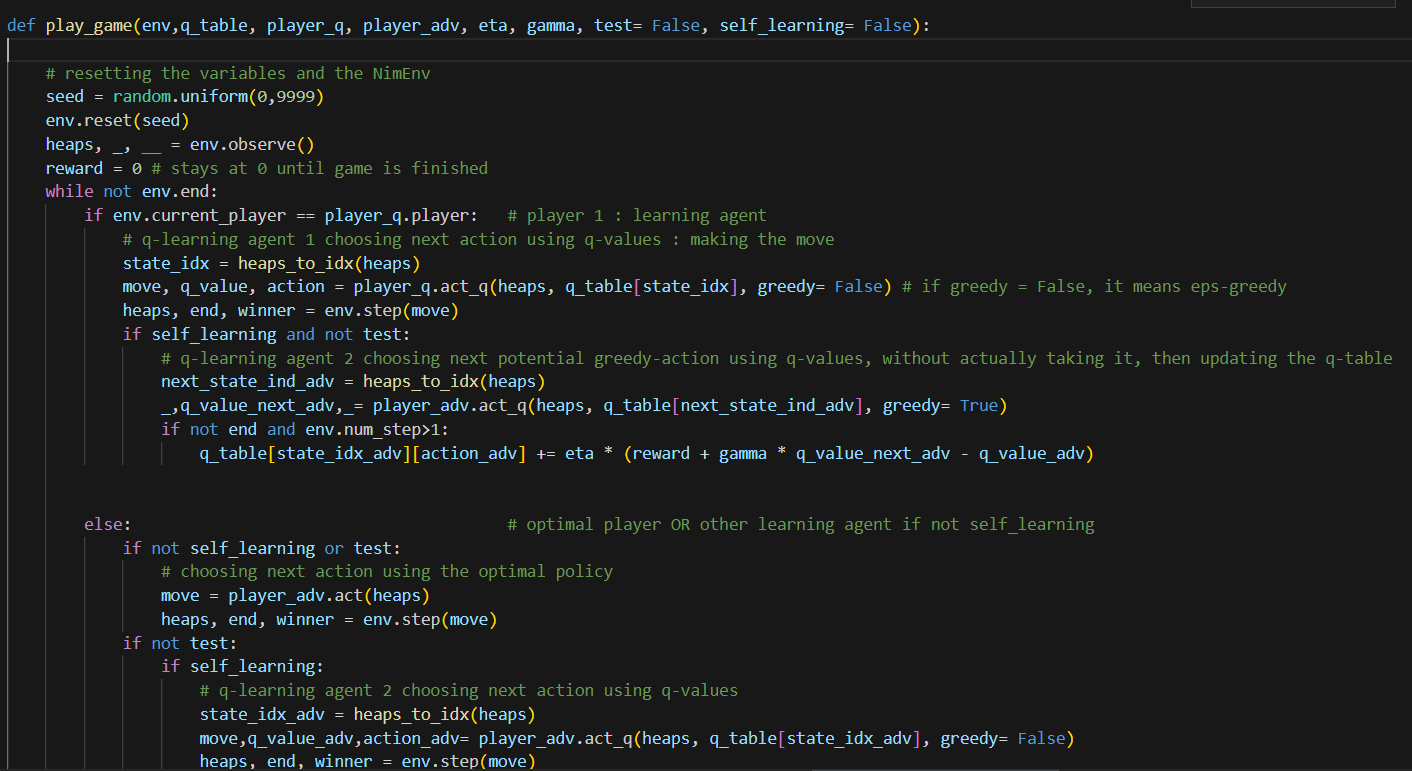
\includegraphics[scale=0.37]{Capture d'écran 2024-06-09 180549}
   \end{figure}
   \end{frame}
      
\begin{frame}{Annexe 2 : code python}
		   \begin{figure}
      \centering
 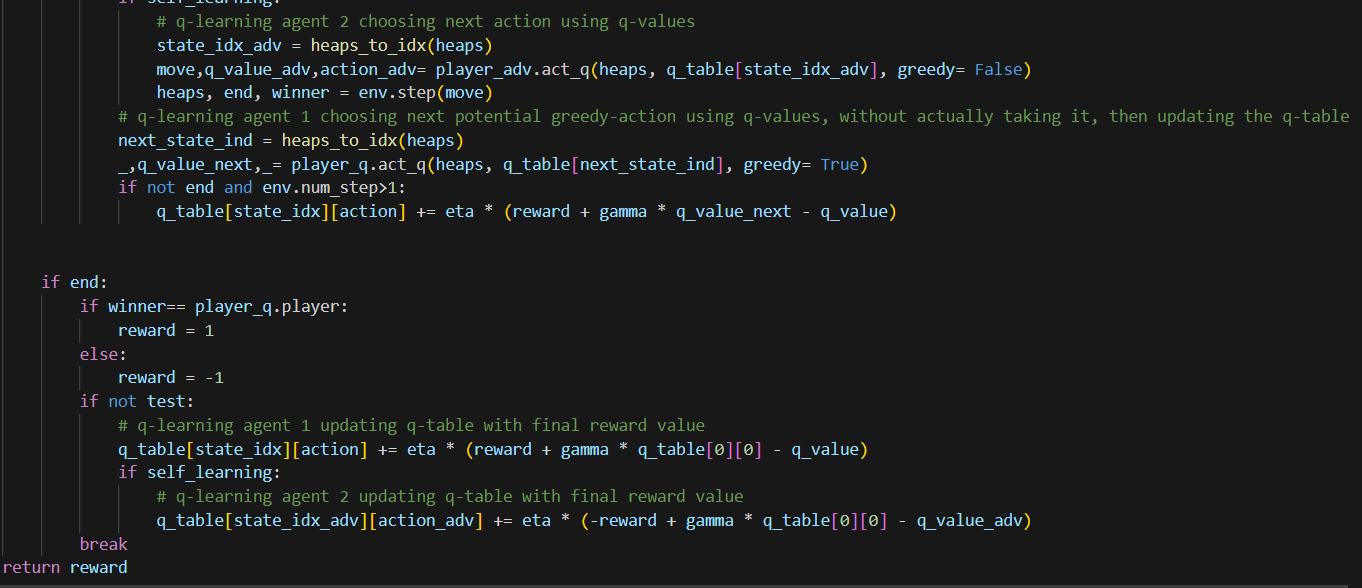
\includegraphics[scale=0.37]{Capture d'écran 2024-06-09 180643}
   \end{figure}
   \end{frame}
   
   \begin{frame}{Annexe 2 : code python}
		   \begin{figure}
      \centering
 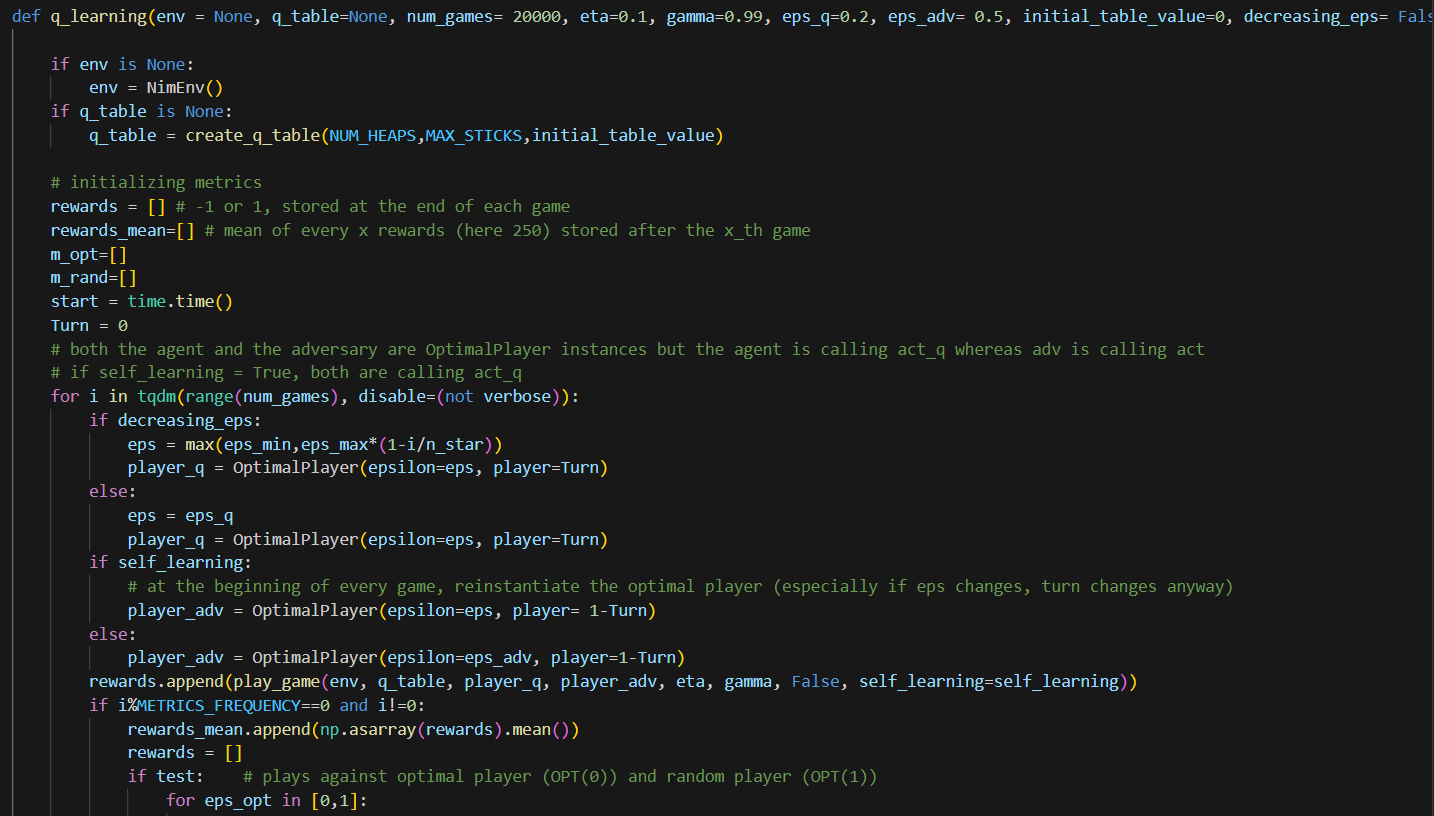
\includegraphics[scale=0.27]{Capture d'écran 2024-06-09 180848}
   \end{figure}
   \end{frame}
   
   \begin{frame}{Annexe 2 : code python}
		   \begin{figure}
      \centering
 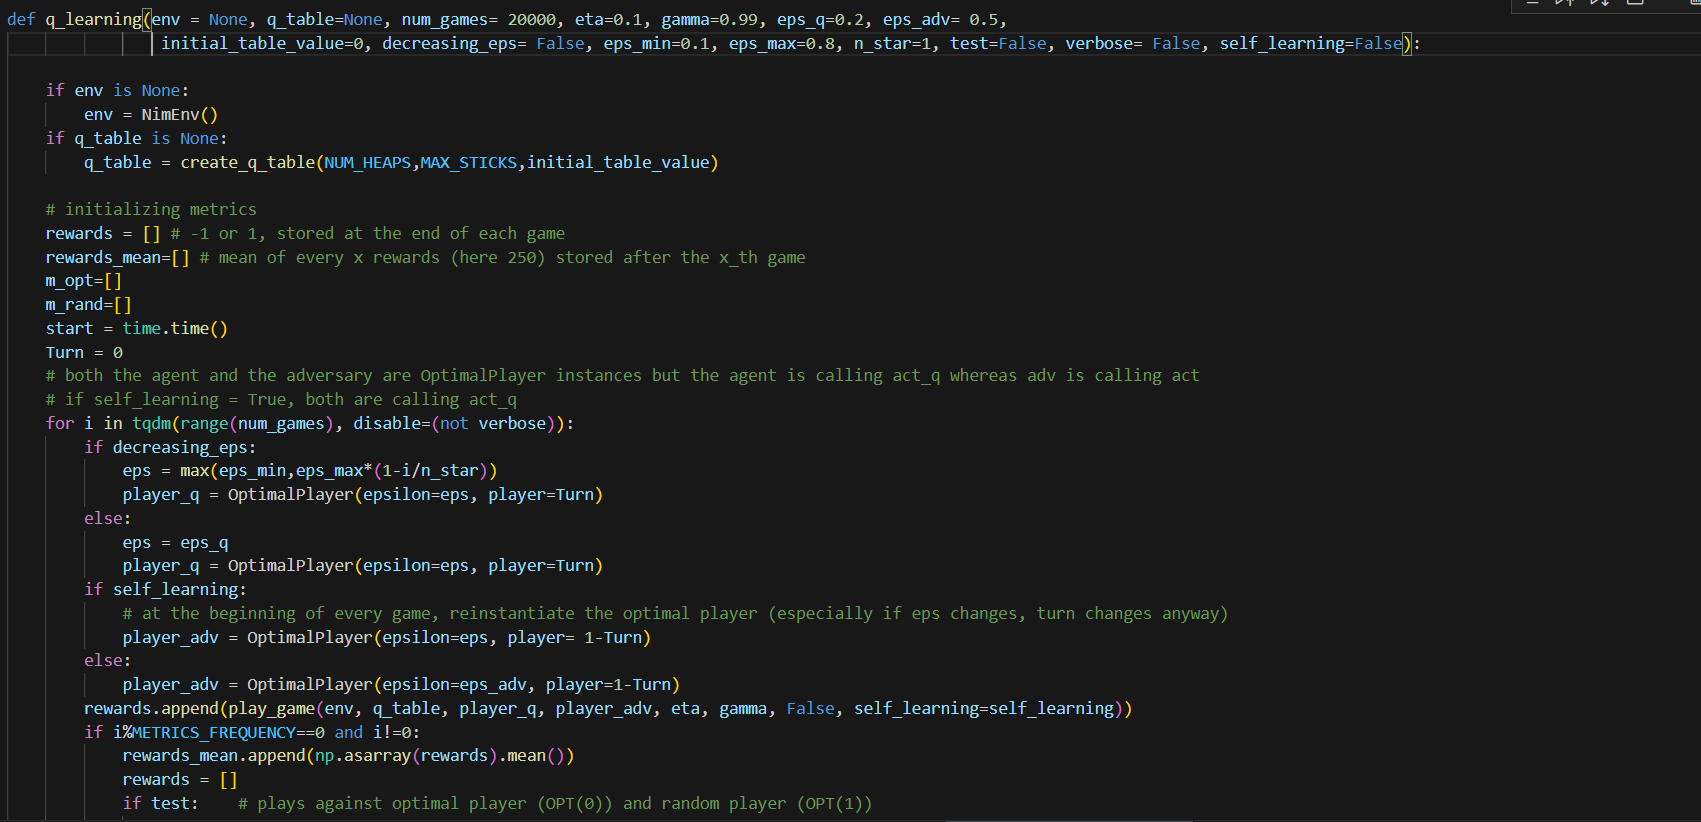
\includegraphics[scale=0.27]{Capture d'écran 2024-06-09 181031}
   \end{figure}
   \end{frame}
   
   \begin{frame}{Annexe 2 : code python}
		   \begin{figure}
      \centering
 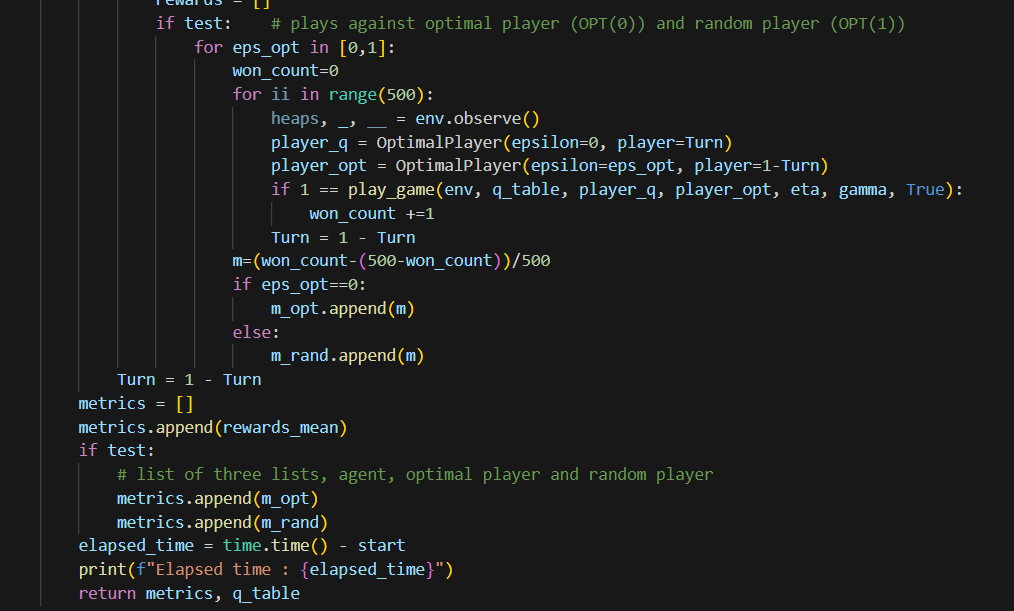
\includegraphics[scale=0.37]{Capture d'écran 2024-06-09 181056}
   \end{figure}
   \end{frame}
   
   \begin{frame}{Annexe 2 : code python}
		   \begin{figure}
      \centering
 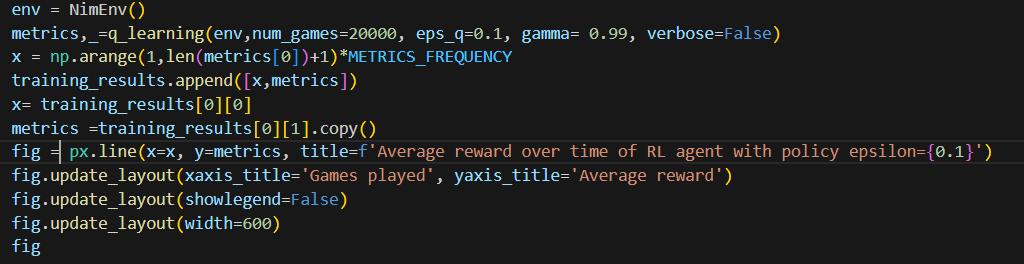
\includegraphics[scale=0.37]{Capture d'écran 2024-06-09 182016}
   \end{figure}
   \end{frame}
\end{document}
